\chapter{Резюме на глава 1: Архитектура на OpenBiodiv}
\label{chapter-openbiodiv}

В тази глава предоставяме архитектурата, т.е. спецификацията и дизайна на OpenBiodiv. Въвеждаме компонентите на OpenBiodiv, които ще бъдат разгледани подробно в следващите глави. Описваме как взаимодействат тези компоненти, за да се формира базираната на знанието система OpenBiodiv.

\section{Какво е OpenBiodiv?}

Разбирането на OpenBiodiv като система базирана на знанието може да се обобщи по следния начин: OpenBiodiv е база данни за взаимосвързана информация за биологичното разнообразие, заедно с логика и приложения, позволяващи на потребителите не само да се допитват до данните, но и да откриват допълнителни факти, свързани с данните. Основните източници на информация в OpenBiodiv са списанията на академичния издател Пенсофт, таксономичната информация от Плаци и таксономичният гръбнак на Global Information Biodiversity Facility (GBIF).

Изследователският проблем на архитектурата на OpenBiodiv може да се формулира като проектиране на семантична графова база данни въз основа на RDF с отворен достъп, включваща информация, предоставяна от Пенсофт, Плаци и GBIF, и позволяваща на потребителите на системата да задават сложни заявки.

OpenBiodiv се състои от (1) семантична графова база данни, (2) програмен код, осигуряващ функционирането на базата и (3) динамична уеб страница (front-end), улесняваща достъпа до основната база от знания (Фиг.~\ref{fig:openbiodiv-components}). OpenBiodiv позволява донамичното вмъкване на данни от хранилища за данни за биологичното разнообразие в текста на статия в Biodiversity Data Journal или друго списание, използващи фреймуорка на Пенсофт за писане на статии, ARPHA-BioDiv (\cite{penev_arpha-biodiv:_2017}). Като втора стъпка, от тези списания се извлича знание, като се възползваме от XML-схемата на тези списания TaxPub. Примерни списания включват ZooKeys, Biodiversity Data Bureau (BDJ), PhytoKeys, MycoKeys и т.н.\footnote{Списанията могат да бъдат достъпвани под \url{https://pensoft.net/browse_journals}}. В същото време факти се извличат от Plazi TreatmentBank, архив на литература за биологичното разнообразие, съдържащ над 200 хиляди таксономични дискусии\footnote{Таксономичната дискусия е специален раздел в биологична публикация, която описва и дискутира вид или по-висок таксон. TreatmentBank е достъпен под \url{https:// //plazi.org/resources/treatmentbank/}} и актуализиран всеки ден. Не на последно място, тези факти са взаимосвързани чрез таксономичният гръбнак на GBIF (\cite{gbif_secretariat_gbif_2017}). След това извлеченото знание се съхранява в базата данни на семантичния граф (Фиг.~\ref{fig:openbiodiv-sources}).

\begin{figure}
\centering
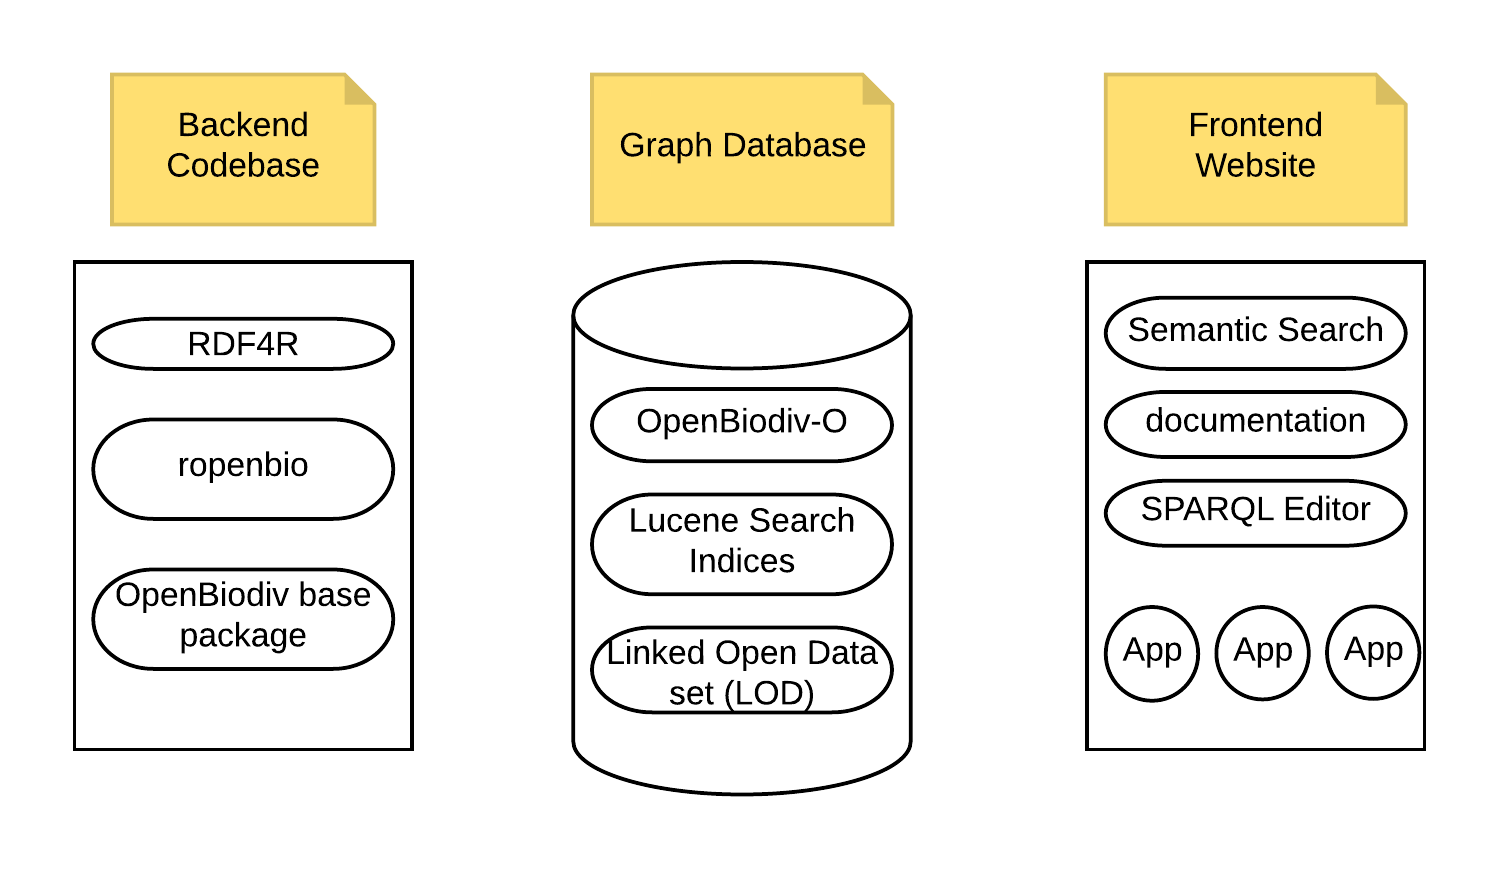
\includegraphics[width=\textwidth]{Figures/components-openbiodiv}
\decoRule
\caption[OpenBiodiv Components]{Компоненти на OpenBiodiv.}
\label{fig:openbiodiv-components}
\end{figure}

\begin{figure}
\centering
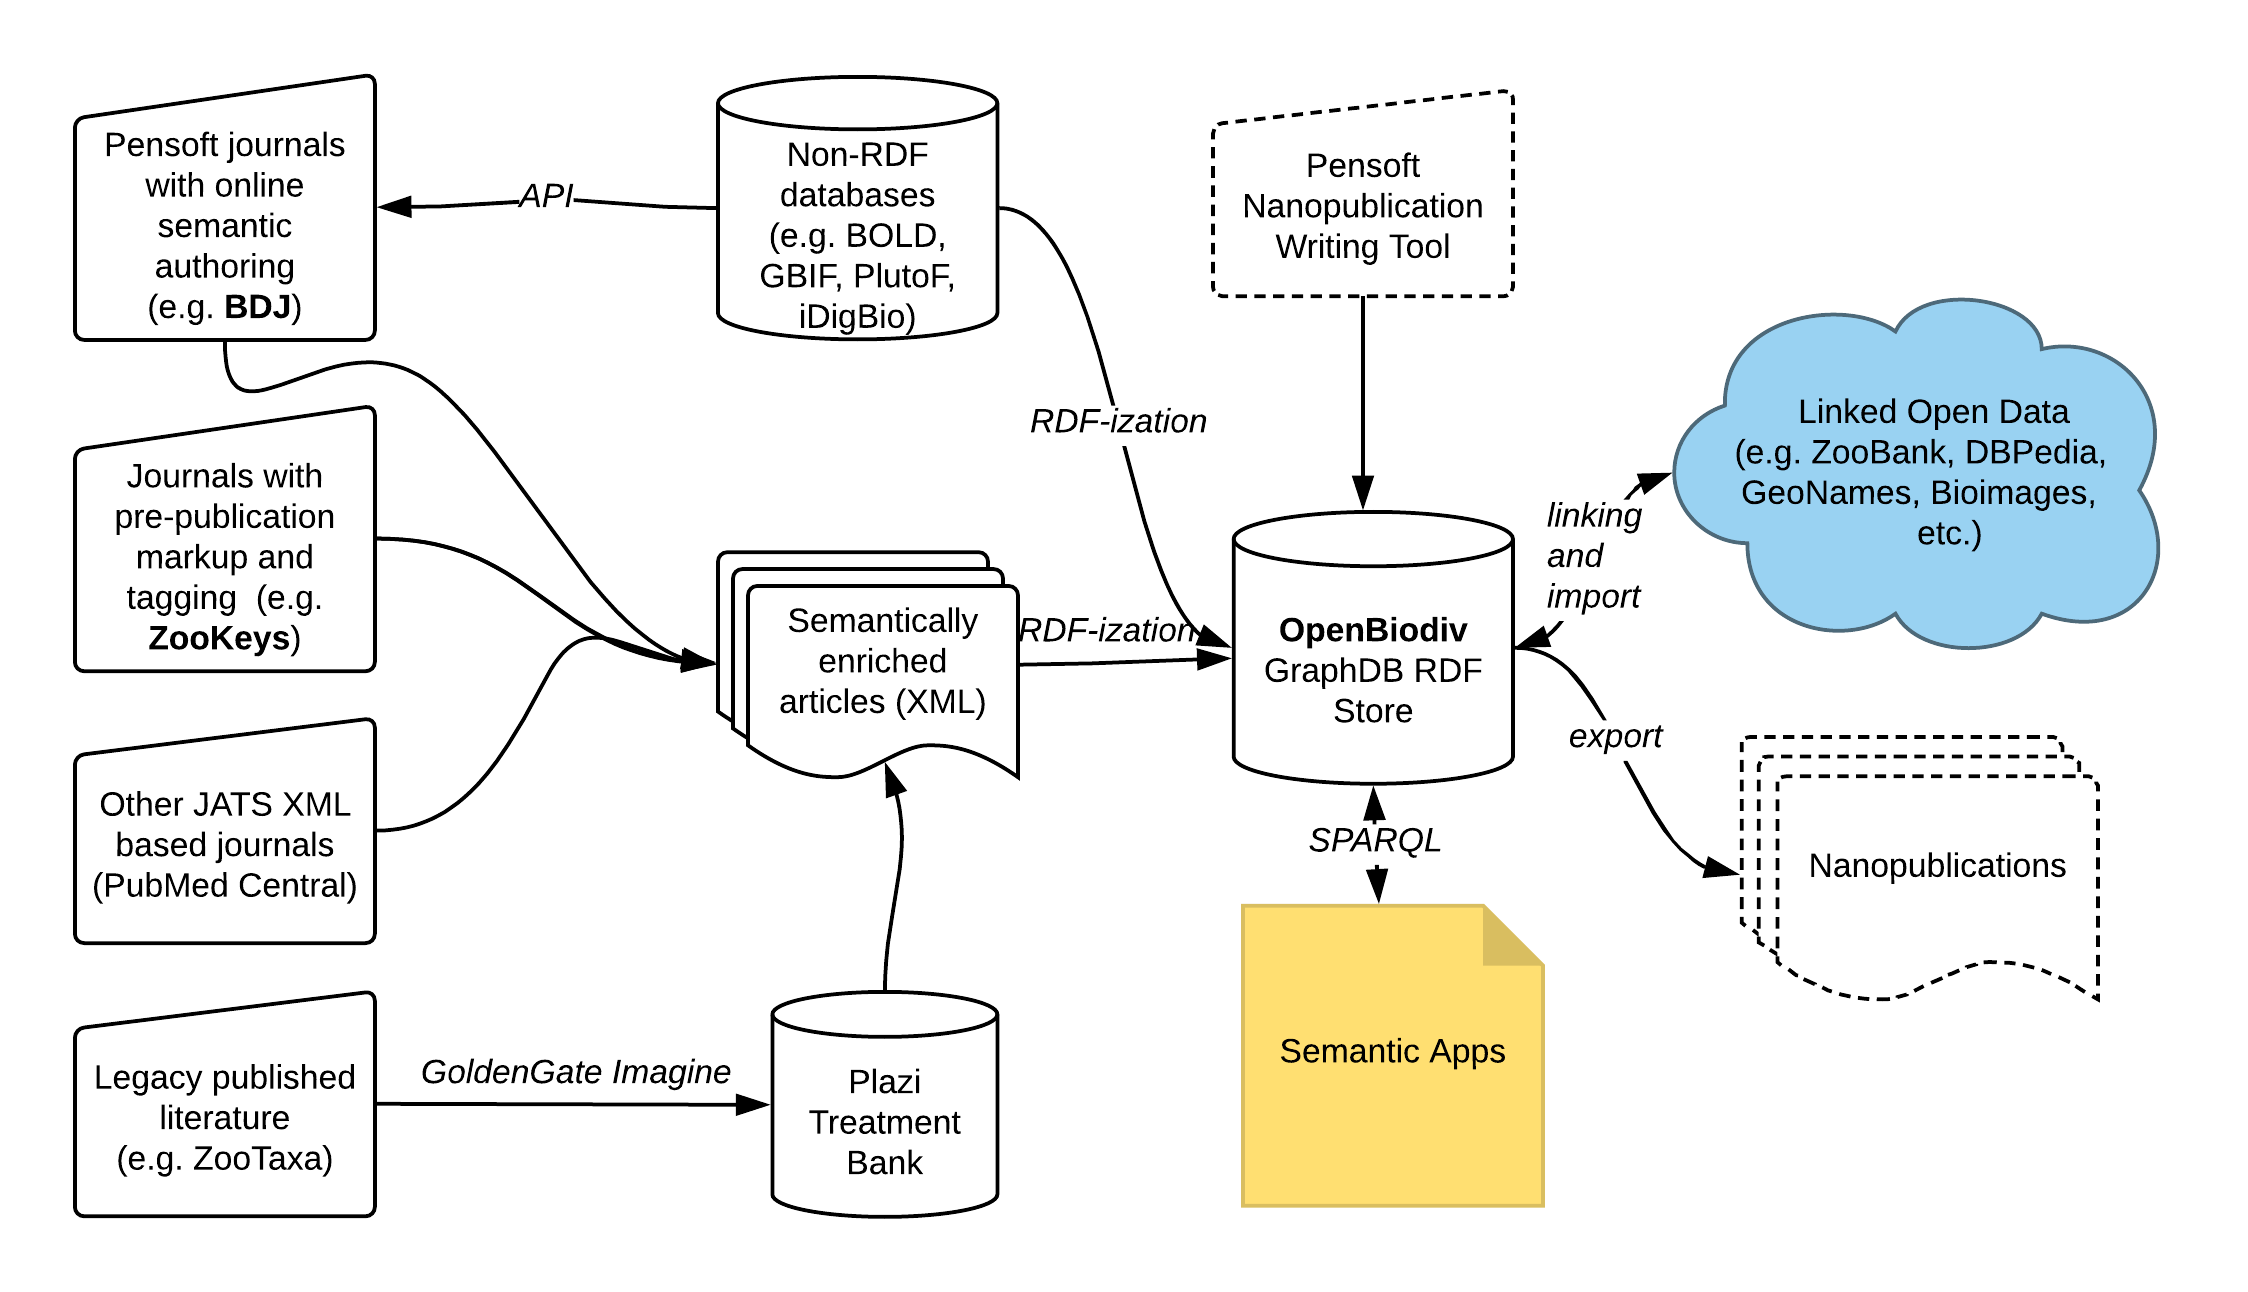
\includegraphics[width=\textwidth]{Figures/openbiodiv-sources}
\decoRule
\caption[OpenBiodiv Components]{Поток на информация в пространството за данни за биологичното разнообразие. Пунктираните линии са компоненти, които все още не са създадени.}
\label{fig:openbiodiv-sources}
\end{figure}

\section{Семантичен граф}

Основен резултат от усилията на OpenBiodiv е създаването на семантична база данни, базирана на знания, извлечени от архивите на Pensoft и Plazi и таксономичния гръбнак на GBIF и достъпни под \url{http://graph.openbiodiv.net/}. Следва обсъждане на компонентите на базата данни.

\subsection{Онтология OpenBiodiv-O}

Централният резултат от усилията по OpenBiodiv е създаването на формален модел на областта за публикуването на знание за биоразнообразието. Този формален модел е онтологията OpenBiodiv-O (\cite{senderov_openbiodiv_2017}). Изходният код на онтологията и придружаващата документация могат да бъдат достъпни под \url{https://github.com/pensoft/openbiodiv-o}. Детайлна дискусия е представена в глава~\ref{chapter-ontology}.

\subsection{Свързани отворени данни OpenBiodiv-LO }

Използвайки OpenBiodiv-O и инфраструктурата, описана по-нататък в тази глава, са създадени свързани отворени данни, включващи приблизително 200 хиляди записа от Плаци, пет хиляди статии от Пенсофт, както и таксономичият гръбнак на GBIF (над милион биологични имена). Данните са достъпни онлайн чрез работния инстумент на семантичната база данни \url{http://graph.openbiodiv.net}. Разясняват се подробно в глава~\ref {chapter-lod}.

\section{Backend}

За да се попълва семантична база данни, е необходимо да се създаде инфраструктура, която преобразува необработени данни (текст, изображения, таблици с данни и т.н.) в структуриран семантичен формат, позволяващ свързването на ресурси посредством техните уникални идентификатори и отговарянето на сложни заявки. OpenBiodiv създаде нова инфраструктура за трансформиране на научни публикации за биоразнообразието в твърдения под формата на RDF с помощта на инструментите, описани в този раздел.

\subsection{RDF4R: R пакет за работа с RDF}

Едно от по-големите технически предизвикателства за OpenBiodiv е трансформирането на информация за биологичното разнообразие (напр. таксономични имена, метаданни, фигури и т.н.), съхранявани като полуструктуриран XML в напълно структурирани семантични знания под формата на RDF. За да се реши това предизвикателство, е разработен R пакет, който позволява създаването, манипулирането и записа в семантична база данни на създадения RDF. Този пакет е достъпен под лиценз с отворен код на GitHub под \url{https://github.com/vsenderov/rdf4r}. Описваме пакета в глава~\ref{chapter-rdf4r}.

\subsection{Базисен програмен код и ROpenBio}

В комбинация с пакета RDF4R, програмният код съдържа още един R пакет, \cl{ropenbio} и базисен програмен код от скриптове и документация, необходими за стартиране на базата данни. \cl{ropenbio} използва пакета RDF4R за преобразуване на полуструктуриран XML в RDF. Той съдържа бийективните проекции, необходими за тази реализация. Той е достъпен под \url{https://github.com/pensoft/ropenbio}. Базисният софтуерен код координира извикването на \cl{ropenbio}, съдържа скриптове за автоматично импортиране на нови ресурси и други подробности. Той е достъпен под \url{https://github.com/pensoft/openbiodiv}. Генерирането на OpenBiodiv-LOD с помощта на тези пакети е обсъдено в глава~\ref{chapter-lod}.

\subsection{Работен процес за преобразуване на екологични метаданни в ръкопис}

Език за екологични метаданни (EML) е популярен формат за описване на екологични данни (\cite{michener_nongeospatial_1997}). Хранилища за биоразнообразие, като GBIF и DataOne, използват този формат, за да опишат набора от данни, които съхраняват. Автоматичното преобразуване на EML файл в data paper ръкопис от Biodiversity Data Journal\footnote {Data paper (\cite{chavan_data_2011}) е научна статия, обсъждаща научни данни.} е възможно с помощта на системата OpenBiodiv (\cite{senderov_online_2016}). Този работен процес е описан подробно в глава~\ref{chapter-case-study}. За да работа в интерактивено режим, отидете на \url{https://arpha.pensoft.net}, влезте в системата (регистрацията е безплатна), изберете ``Start a new manuscript'', превъртете до ``Import manuscript'' и следвайте необходимите стъпки, за да качите EML файл и да го използвате като шаблон за вашия нов ръкопис.

\subsection{Работен процес за импортиране на данни за наблюдения на видове в ръкопис}

Един от важните видове данни за биологичното разнообразие са данни за наблюдения на организми occurrence data. Това са данни, които документират наличието на правилно таксономично идентифициран организъм на дадено място и време. Такива данни се съхраняват в международни хранилища като BOLD, GBIF, PlutoF и iDigBio. За да се улесни публикуването на такъв тип данни е разработен работен процес за импортиране на записи за събития от тези бази данни в таксономична статия в списанието Biodiverstiy Data Journal (\cite{senderov_online_2016}). Този работен процес е описан подробно в глава~\ref{chapter-case-study}. За да отворите интерактивно работния процес, отидете на \url{https://arpha.pensoft.net}, влезте в системата (регистрацията е безплатна), изберете ``Start a new manuscript'', изберете ``Biodiveristy Data Journal'', ``Taxonomic paper''  и ``Create a new manuscript''. След това в новия ръкопис щракнете с мишката върху раздела ``Taxon treatments'', като кликнете върху знака $+$ до него, и укажете биологичната класификация на новия запис (напр. Animalia), и най-накрая щракнете върху ``Save'' и ще ви бъде представен избор на подраздели. Кликнете върху секцията ``Materials'' от-вляво, за да видите инструмента на работния процес за вмъкване на материли. Погледнете в долната част на диалоговия прозорец, където можете да поставите множество идентификационни номера. Това е частта, в която избирате външни идентификатори на ресурси, които да бъдат импортирани във вашата статия.

\section{Интерфейс}

В допълнение към предоставянето endpoint за база данни с възможност за търсене, се разработва уебсайт, позволяващ семантично търсене и капсулиращ специфични задачи, пакетирани като приложения (\url{http://openbiodiv.net}). Развитието на сайта надхвърля обхвата на дисертационната теза и се ръководи от екипа за разработка на Пенсофт. Бета версията вече е в действие. Фиг.~\ref{fig:website}. Ограничена дискусия е представена в глава~\ref{webportal}.

\section{Системна администрация}

Системата е разположена на виртуална машина на Debian GNU+Linux. GraphDB работи с heap файл от 20 ГБ и с набор от правила RDFS-Plus Optimized\footnote{Това се налага поради факта, че достигнахме препятствия, когато използвахме OWL извод. Обсъдени в глава~\ref {chapter-lod}}. Непрекъснатата работа се осигурява от автоматичното изпълнение на скриптове от директорията \cl{run} на базисния код на OpenBiodiv.

\begin{figure}
\centering
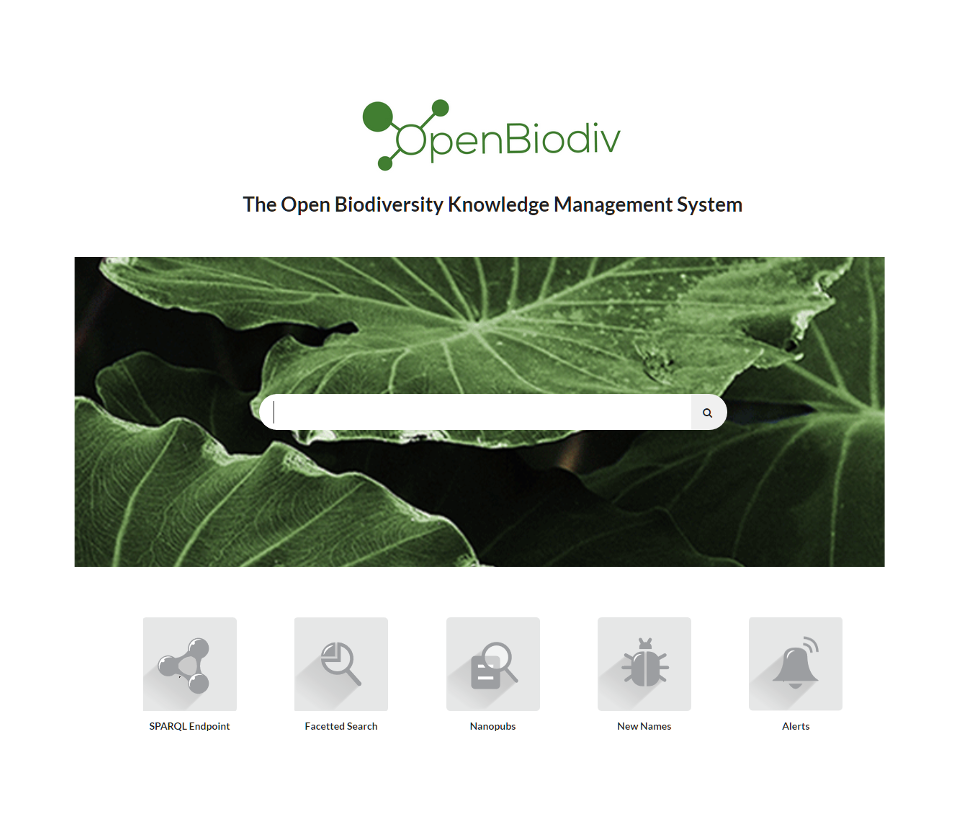
\includegraphics[width=\textwidth]{Figures/openbiodiv-webpage}
\decoRule
\caption[OpenBiodiv Website]{Бета версия на потребителския интерфейс.}
\label{fig:website}
\end{figure}


